\documentclass[border=10pt]{standalone}
\usepackage{tikz}
\usetikzlibrary{calc,positioning,shadows.blur,decorations.pathreplacing}
\usepackage{etoolbox}
\usepackage{graphicx}
\usepackage{amsmath}
\graphicspath{{/home/jake/Documents/MOSES/MCOR/python/}}

\begin{document}
	\begin{tikzpicture}
	
	%begin by adding a node for each figure
	\node[inner sep=0pt] (fig1) at (0,0)
		{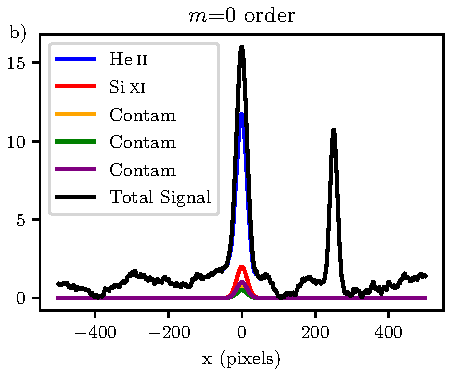
\includegraphics[]{fig1}};
	\node[inner sep=0pt] (fig2) at (0,2.7)
		{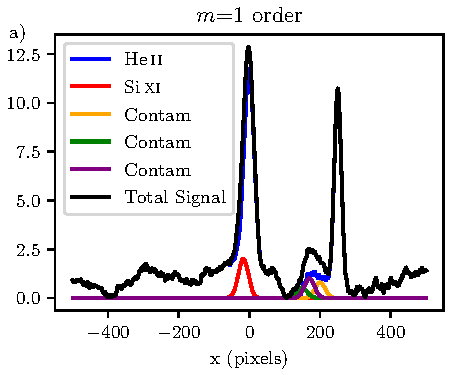
\includegraphics[]{fig2}};
	\node[inner sep=0pt] (fig3) at (0,-2.7)
		{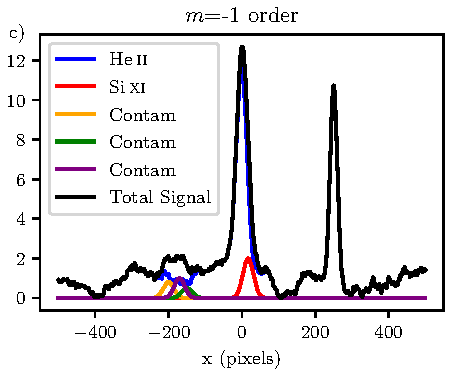
\includegraphics[]{fig3}};
%	\node[inner sep=0pt] (fig4) at (4,1.5)
%		{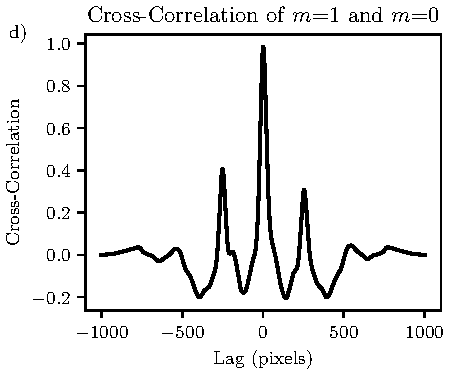
\includegraphics[width=.25\textwidth]{fig4}};
%	\node[inner sep=0pt] (fig5) at (4,-1.5)
%		{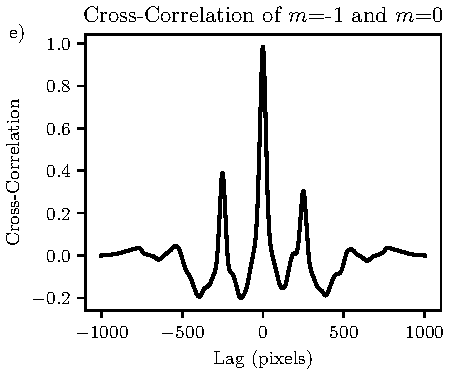
\includegraphics[width=.25\textwidth]{fig5}};
	\node[inner sep=0pt] (fig6) at (3.6,2.7)
		{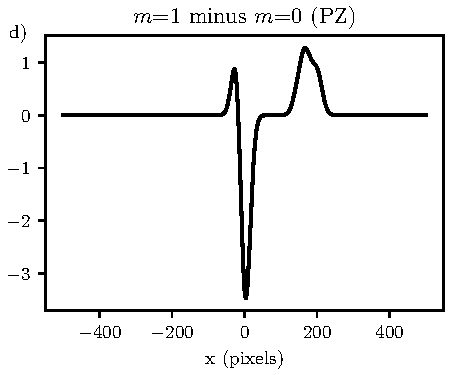
\includegraphics[]{fig6}};
	\node[inner sep=0pt] (fig7) at (3.6,0)
		{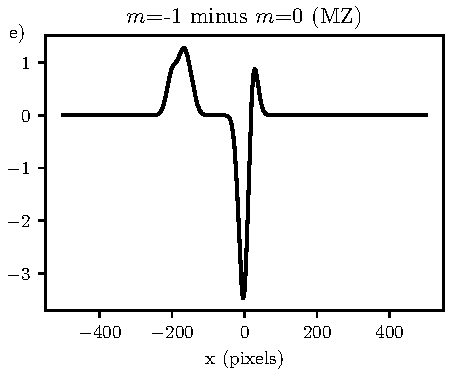
\includegraphics[]{fig7}};
	\node[inner sep=0pt] (fig8) at (3.2,-2.7)
		{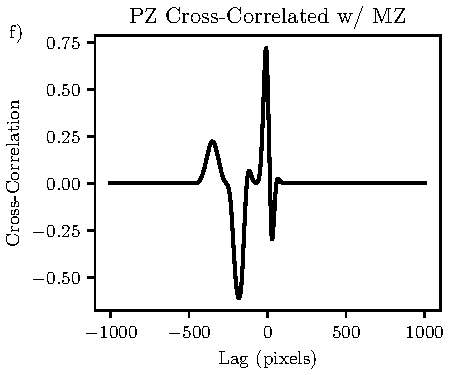
\includegraphics[]{fig8}};
		
	%add symbol for operation
	\node[inner sep=0pt](dif1) at (1.8,+2.5)
		{$\boldsymbol{\bigtriangleup}$};
	\node[inner sep=0pt](dif2) at (1.8,0)
		{$\boldsymbol{\bigtriangleup}$};
	\node[inner sep=0pt](cc1) at (5.1,-2.5)
		{$\bigotimes$};
	\node[inner sep=0pt](t1) at (5.5,2.5)
		{};
	\node[inner sep=0pt](t2) at (5.5,-2.5)
		{};
		
		
	%lets try drawing some lines between them.
	\draw[->] (fig1.north east) -- (dif1.south);
	\draw[->] (fig2.east) -- (dif1.west);
	\draw[->] (dif1.east) -- (fig6.west);
	
	\draw[->] (fig1.east) -- (dif2.west);
	\draw[->] (fig3.north east) -- (dif2.south);
	\draw[->] (dif2.east) -- (fig7.west);
	
	\draw[->] (fig6.east) -- (t1);
	\draw[->] (t1) -- (t2);
	\draw[->] (t2) -- (cc1.east);
	\draw[->] (cc1.west) -- (fig8.east);
	\draw[->] (fig7.east) -- (cc1.north);
	
%	\draw[->] (fig2.south) -- (dif1.north);
%	\draw[->] (fig3.south) -- (dif2.north);
%	\draw[-] (fig1.south) -- (mid);
%	\draw[->] (mid) -- (dif1.west);
%	\draw[->] (mid) -- (dif2.east);
%	\draw[->] (dif2.south) -- (fig7.north);
%	\draw[->] (dif1.south) -- (fig6.north);
%	
%	\draw[->] (-2.5,-5.4) -- (cc3.west);
%	\draw[->] (2.5,-5.4) -- (cc3.east);
%	\draw[->] (cc3.south) -- (fig8.north);
	
	%draw a symbol legend
	\node(align)[draw] at (2,-4.5) {
		\begin{tabular}{c}
		\tiny{$\bigotimes$ = Cross-Correlation} \\
		\tiny{$\boldsymbol{\bigtriangleup}$ = Difference}
		\end{tabular}};

	
	\end{tikzpicture}
\end{document}